 \documentclass[12pt]{article}
\usepackage{polski}
\usepackage[utf8]{inputenc}
\usepackage{graphicx}
\usepackage{listings}
\usepackage{color}

\definecolor{dkgreen}{rgb}{0,0.6,0}
\definecolor{gray}{rgb}{0.5,0.5,0.5}
\definecolor{mauve}{rgb}{0.58,0,0.82}

\lstset{frame=tb,
  aboveskip=3mm,
  belowskip=3mm,
  showstringspaces=false,
  columns=flexible,
  basicstyle={\small\ttfamily},
  numbers=none,
  numberstyle=\tiny\color{gray},
  keywordstyle=\color{blue},
  commentstyle=\color{dkgreen},
  stringstyle=\color{mauve},
  breaklines=true,
  breakatwhitespace=true,
  tabsize=3
}


\begin{document}

\begin{titlepage}
\centering

\includegraphics[width=0.15\textwidth]{logo}\par\vspace{1cm}
{\scshape\LARGE Politechnika Warszawska \par}
\vspace{1cm}
{\huge\bfseries  Projekt techniczny \linebreak \\ Aplikacja do gry w szachy z wykorzystaniem komunikacji webowej oraz interfejsu graficznego 3D \par}
\vspace{1cm}
{\bfseries Projekt Indywidualny \par}
\vspace{2cm}
{\Large\itshape  Sebastian Kurpios \par}
\end{titlepage}

\tableofcontents
\newpage

\section{Opis aplikacji}
Celem projektu jest wykonanie aplikacji do gry w szachy z interfejsem 3D. Program powinien pozwalać na grę jednoosobową z możliwością wyboru stopnia trudności oraz wieloosobową. Dodatkowo wersja wieloosobowa powinna umożliwić komunikację pomiędzy graczami oraz wybór gracza według jego umiejętności. Ponadto użytkownik aplikacji będzie mógł zarejestrować się w serwisie, a wyniki jego potyczek będą zapisywane w bazie danych.  

\section{Komponenty}
\begin{enumerate}
\item Aplikacja desktopowa - klient
\item Serwer komunikacyjny
\item Serwer bazy danych
\end{enumerate}

\begin{figure}[!ht]
  \centering
	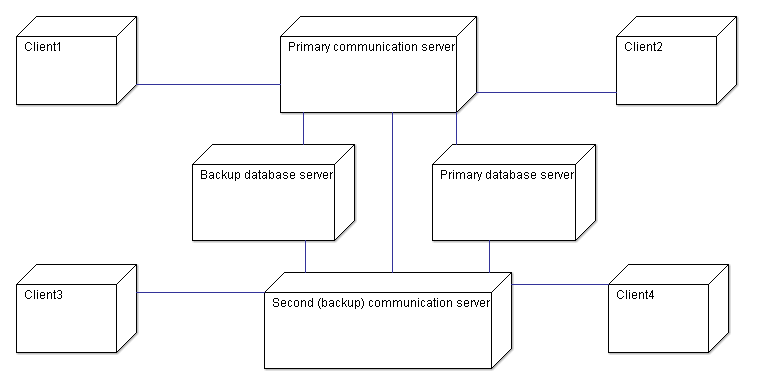
\includegraphics[scale=0.60]{DeploymentDiagram}
  \caption{Diagram komponentów}
\end{figure}

\section{Dane wejściowe i wyjściowe}
\subsection{Dane wejściowe}
\begin{enumerate}
\item Dane wejściowe (konfiguracyjne) serwera
\begin{itemize}
\item Port nasłuchiwania
\item Nazwa bazy danych
\item Nazwa użytkownika bazy danych
\item Hasło bazy danych
\end{itemize}
\item Dane wejściowe aplikacji klienckiej
\begin{itemize}
\item Dane początkowe i konfiguracyjne
\begin{enumerate}
\item Adres IP serwera
\item Port serwera
\item Tryb gry
\item Dane kamery
\end{enumerate}
\item Dane logowania 
\begin{enumerate}
\item Login
\item Hasło
\end{enumerate}
\item Dane rejestracji
\begin{enumerate}
\item Login
\item Hasło
\item Adres E-mail
\item Imię
\item Nazwisko
\end{enumerate}
\item Dane aplikacji w trybie jednoosobowym
\begin{enumerate}
\item Algorytm działania
\item Poziom trudności
\end{enumerate}
\item Dane aplikacji w trybie wieloosobowym
\begin{enumerate}
\item Identyfikator wybranego przeciwnika
\item Tryb komunikacji pomiędzy użytkownikami (kamera czy komunikator tekstowy)
\end{enumerate}
\end{itemize}
\end{enumerate}

\subsection{Dane wyjściowe}
\begin{enumerate}
\item Dane wyjściowe serwera - brak, serwer nie kończy działania
\item Dane wyjściowe aplikacji klienckiej
\begin{itemize}
\item Wynik gry
\item Liczba punktów zdobytych za grę
\item Uaktualniony ranking
\end{itemize}
\end{enumerate}

\newpage

\section{Wymagania}
\subsection{Diagram użycia}

\begin{figure}[!ht]
  \centering
	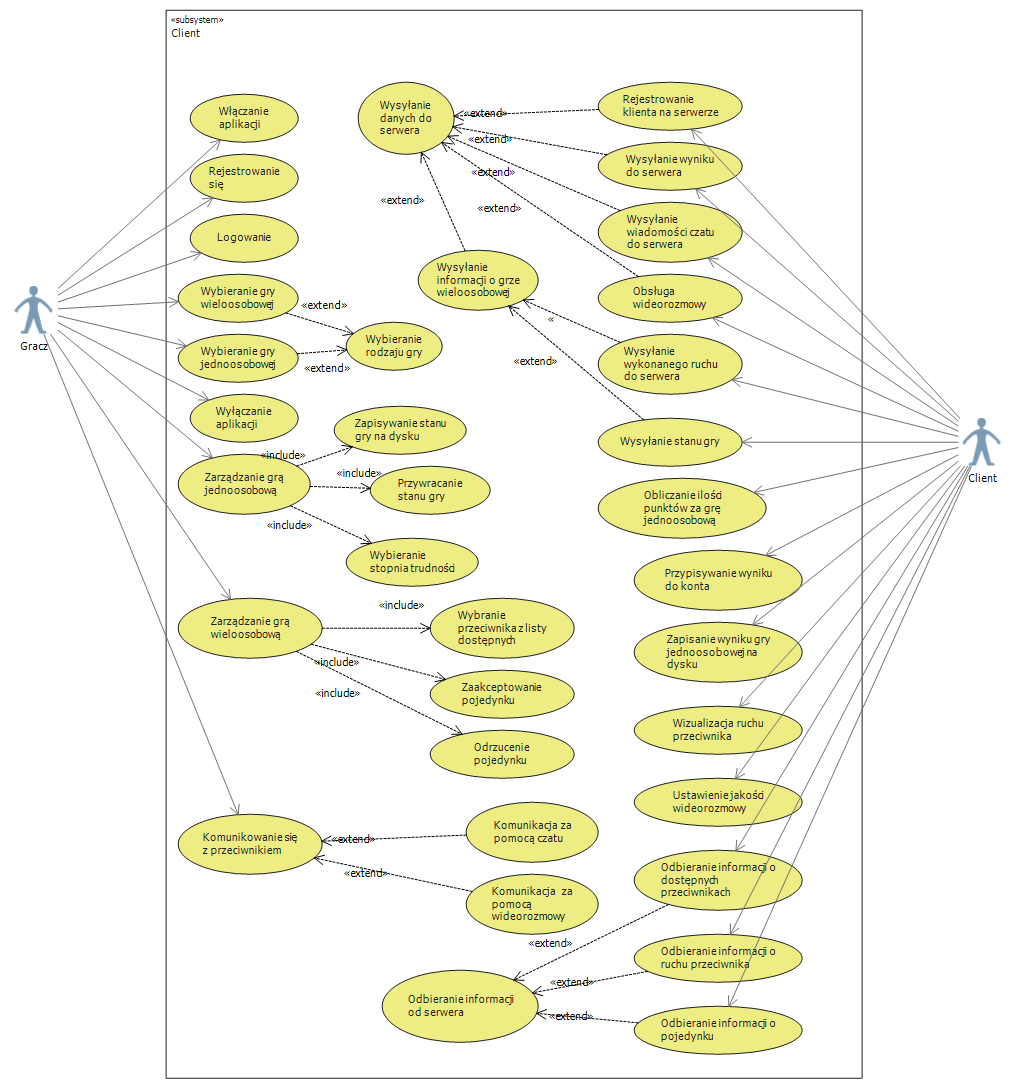
\includegraphics[scale=0.5]{clientUseCase}
	 \caption{Diagram użycia dla aplikacji klienckiej}
\end{figure}

\newpage

\begin{figure}[!ht]
  \centering
	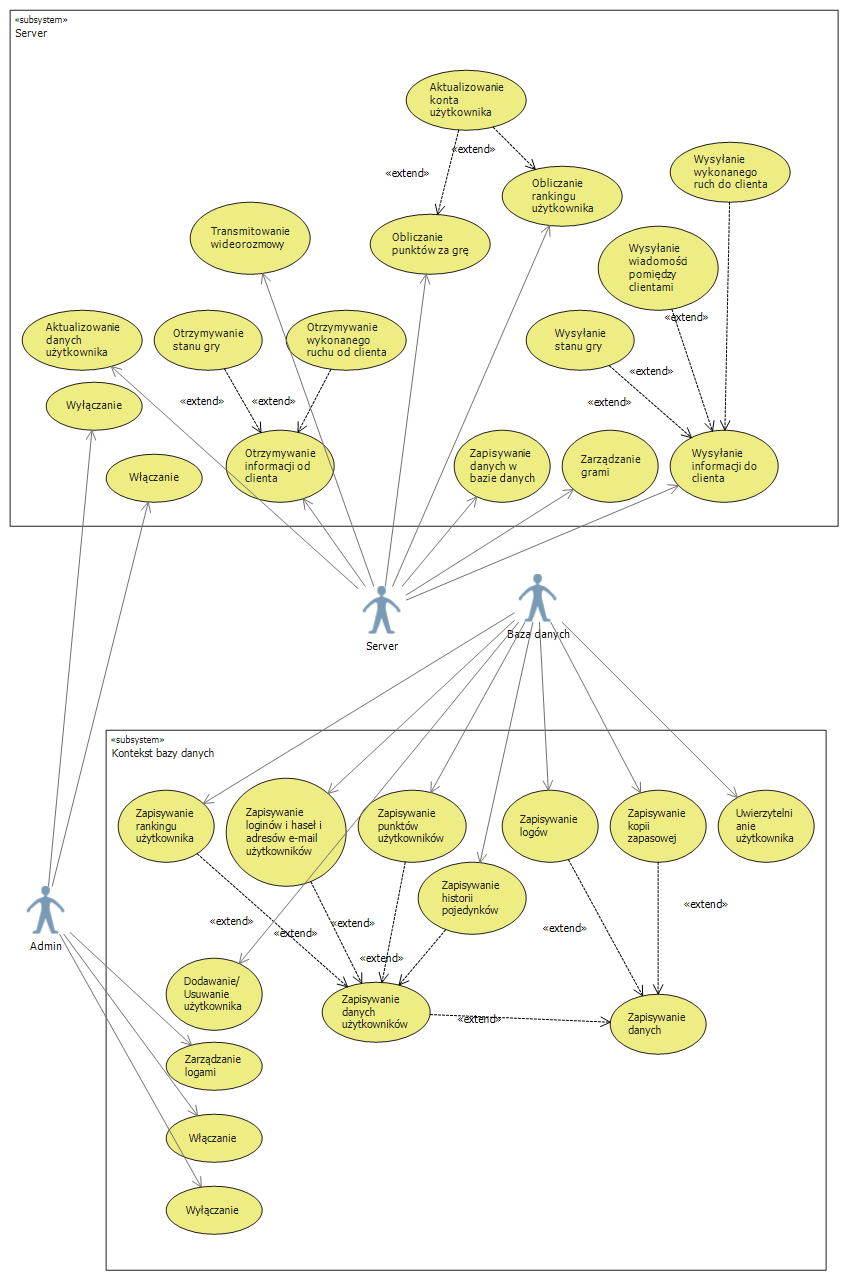
\includegraphics[scale=0.5]{serverUseCase}
	 \caption{Diagram użycia dla serwera i bazy danych}
\end{figure}

\subsection{Wymagania funkcjonalne}
\begin{enumerate}
\item Gra jednoosobowa:
\begin{itemize}
\item wybieranie stopnia trudności wirtualnego przeciwnika (głębokość dla algorytmu min-max lub alfa-beta)
\item zapisywanie stanu gry i przywracanie go w dowolnym momencie
\item obliczanie ilości punktów za grę ze względu na trudność przeciwnika i wynik
\item zapisywanie na dysku wyniku gry oraz liczby otrzymanych punktów 
\item przypisywanie liczby otrzymanych punktów do danego konta
\end{itemize}

\item Gra wieloosobowa:
\begin{itemize}
\item wybieranie przeciwnika z listy dostępnych użytkowników
\item możliwość akceptacji lub odrzucenia zaproponowanego pojedynku przez innego użytkownika  
\item możliwość komunikacji z przeciwnikiem za pomocą czatu lub wideorozmowy
\item obliczanie ilości punktów za grę ze względu na ranking przeciwnika i wynik
\item możliwość rozgrywania gry anonimowo lub jako zalogowany użytkownik
\item możliwość identyfikacji użytkownika za pomocą konta w serwisie facebook
\end{itemize}
\end{enumerate}

\subsection{Wymagania niefunkcjonalne}
\begin{enumerate}
\item Reakcja na niedostępność serwera z powodu awarii lub braku odpowiedzi na zapytanie w wyznaczonym czasie:
\begin{itemize}
\item możliwość rozegrania gry wyłącznie w trybie z komputerem
\item brak możliwości dopisania liczby otrzymanych punktów do konta gracza
\item zapisanie stanu gry wyłącznie na dysku
\item w razie przerwania gry automatyczne zakończenie pojedynku bez przyznania punktów 
\end{itemize}

\item Reakcja na przerwanie połączenia z klientem w czasie gry
\begin{itemize}
\item oczekiwanie przez wyznaczony czas na użytkownika
\item przyznanie przegranej niedostępnemu użytkownikowi po odczekaniu
\end{itemize}

\item Reakcja na brak urządzeń audio-wideo w urządzeniu użytkownika
\begin{itemize}
\item brak możliwości komunikacji za pomocą wideorozmowy
\end{itemize}
\end{enumerate}


\newpage
\section{Schematy blokowe}
\begin{figure}[!ht]
  \centering
	\includegraphics[scale=0.5]{clientLoginBlock}
	 \caption{Schemat blokowy logowanie i rejestracji}
\end{figure}
\pagebreak
\begin{figure}[!ht]
  \centering
	\includegraphics[scale=0.4]{clientBlock}
	 \caption{Uproszczony schemat blokowy aplikacji klienckiej}
\end{figure}

\newpage

\section{Diagram klas}

\begin{figure}[!ht]
  \centering
	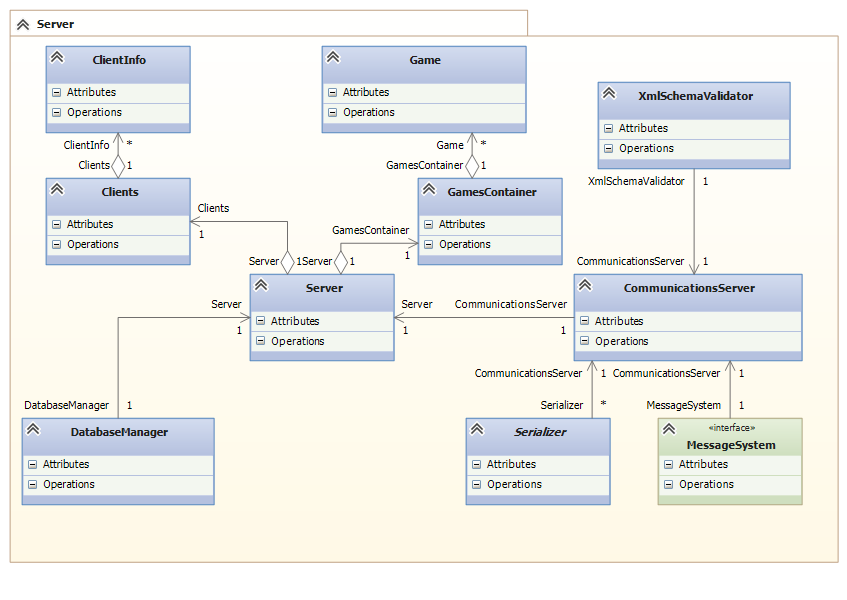
\includegraphics[scale=0.7]{serverClassDiagram}
	 \caption{Diagram klas dla serwera}
\end{figure}

\newpage

\begin{figure}[!ht]
  \centering
	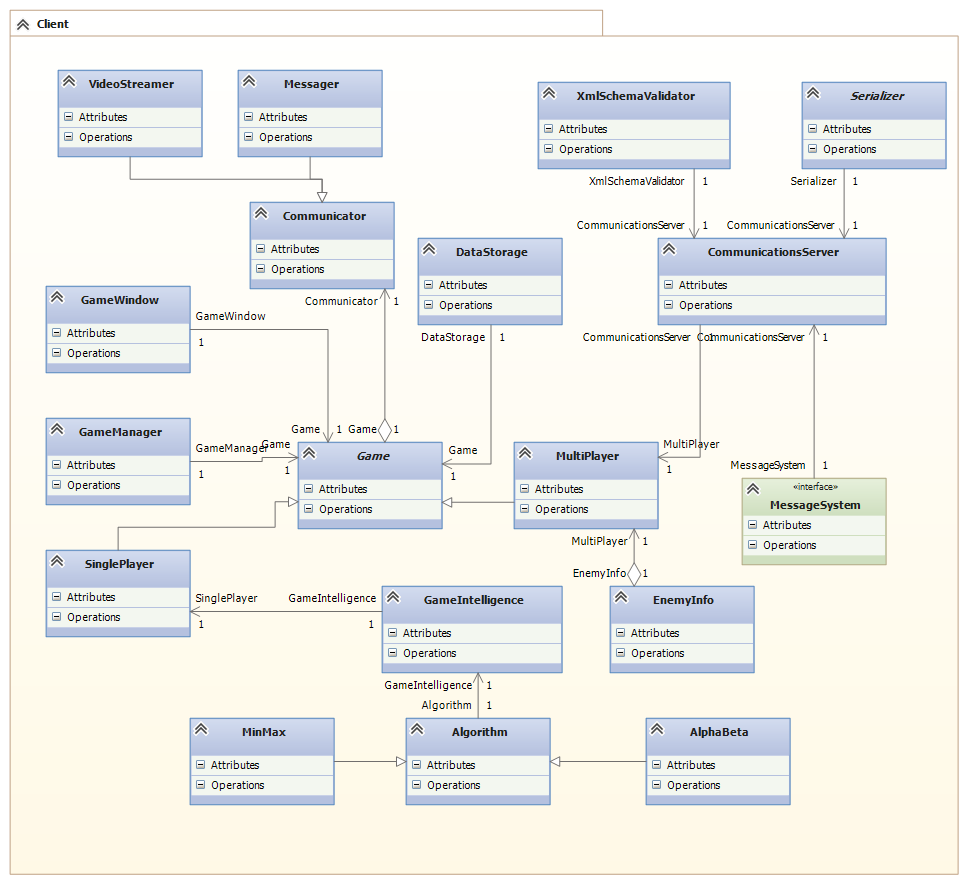
\includegraphics[scale=0.6]{clientClassDiagram}
	 \caption{Diagram klas dla aplikacji klienckiej}
\end{figure}

\newpage

\section{Diagram związków encji}
\begin{figure}[!ht]
  \centering
	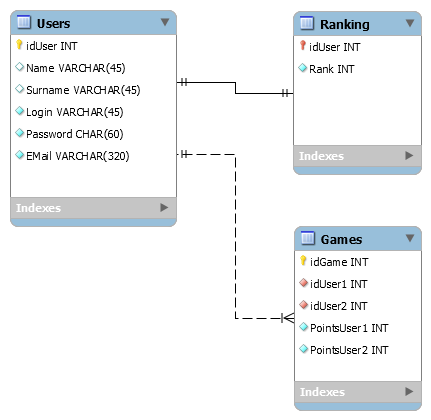
\includegraphics[scale=0.6]{erd}
	 \caption{Diagram związków encji bazy danych}
\end{figure}

\section{Technologia}
\begin{enumerate}
\item Język programowania - C\#
\item Platforma - .Net Framework 
\begin{itemize}
\item Dostęp do bazy danych - ADO.NET
\item Komunikacja - Gniazda sieciowe
\item Interfejs graficzny (GUI) - Windows Forms
\end{itemize}
\item Silnik graficzny - OpenTK
\item Baza danych - Microsoft SQL Server
\end{enumerate}


\section{Algorytmy}
\subsection{Algorytm min-max}
\begin{lstlisting}
function minimax(wezel, glebokosc, maxGracz)
    if glebokosc = 0 or wezel jest terminalny
        return heurystyke w wezle

     if maxGracz
         najlepszaWartosc = -inf
        for each dziecka wezla
             v = minimax(dziecko, glebokosc-1, FALSE)
             najlepszaWartosc = max(najlepszaWartosc, v)
         return najlepszaWartosc

     else    (* minGracz *)
        najlepszaWartosc = -inf
        for each dziecka wezla
         v = minmax(dziecko, glebokosc-1, TRUE)
           najlepszaWartosc = min(najlepszaWartosc, v)
       return najlepszaWartosc

\end{lstlisting}

\subsection{Algorytm alfa-beta}
\begin{lstlisting}
funkcja alfabeta(wezel, glebokosc, alfa, beta)
    if wezel jest koncowy lub glebokosc = 0
        return wartosc heurystyczna wezla
        
    if przeciwnik ma zagrac w wezle
        for each potomka wezla
            beta = min(beta, alfabeta(potomek, glebokosc-1, alfa, beta))
            if alfa >= beta
                przerwij przeszukiwanie  {odcinamy galaz Alfa}
        return beta
    else {my mamy zagrac w wezle}
        foreach potomka wezla
            alfa = max(alfa, alfabeta(potomek, glebokosc-1, alfa, beta))
            if alfa >= beta
                przerwij przeszukiwanie  {odcinamy galaz Beta}
        return beta

\end{lstlisting}

\subsection{Analiza istniejących rozwiązań}
\subsubsection{Przykłady istniejących programów}
\begin{itemize}
\item Arena \footnote{http://www.playwitharena.com/}
\item WinBoard \footnote{http://hgm.nubati.net/}
\item Chessmaster 11th Edition \footnote{http://chessmaster.uk.ubi.com/xi/index.php}
\end{itemize}

Większość aplikacji do gry w szachy posiada albo rozbudowany interfesj graficzny albo rozbudowany dostęp do silników graficznych, a aplikację, które mają te dwie cechy są zazwyczaj płatne. Moja aplikacja do gry w szachy będzie łączyć te dwie cechy wraz z rozbudowaną komunikacją pomiędzy użytkownikami, a ponadto będzie opensource.

\end{document}